\tikzset{every picture/.style={line width=0.75pt}} %set default line width to 0.75pt        

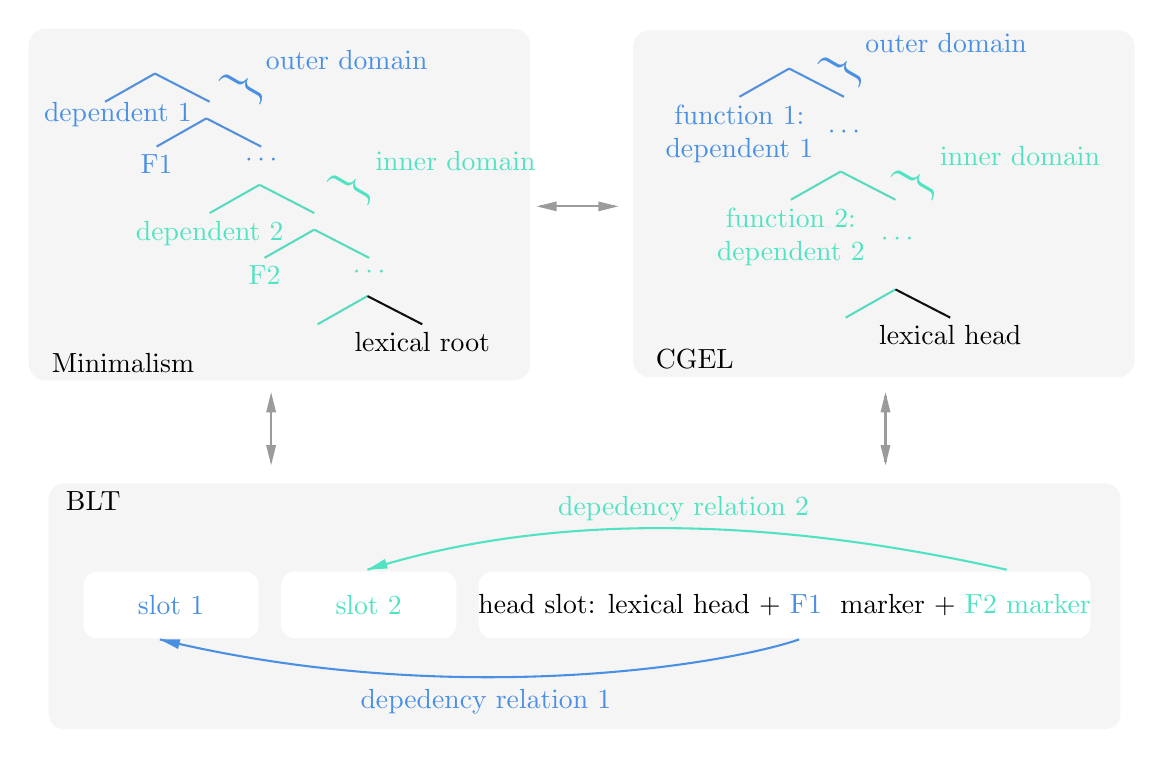
\begin{tikzpicture}[x=0.75pt,y=0.75pt,yscale=-0.8,xscale=0.8]
%uncomment if require: \path (0,559); %set diagram left start at 0, and has height of 559

%Straight Lines [id:da49162210331654554] 
\draw [color={rgb, 255:red, 80; green, 227; blue, 194 }  ,draw opacity=1 ]   (226,174) -- (256,157) ;
%Straight Lines [id:da6822202220492657] 
\draw [color={rgb, 255:red, 80; green, 227; blue, 194 }  ,draw opacity=1 ]   (289,174) -- (256,157) ;
%Straight Lines [id:da5610373452641617] 
\draw [color={rgb, 255:red, 80; green, 227; blue, 194 }  ,draw opacity=1 ]   (258,214) -- (288,197) ;
%Straight Lines [id:da8651773913180412] 
\draw    (321,214) -- (288,197) ;
%Straight Lines [id:da10480931775332558] 
\draw [color={rgb, 255:red, 74; green, 144; blue, 226 }  ,draw opacity=1 ]   (161,107) -- (168.67,102.65) -- (191,90) ;
%Straight Lines [id:da8781100694963793] 
\draw [color={rgb, 255:red, 74; green, 144; blue, 226 }  ,draw opacity=1 ]   (224,107) -- (191,90) ;
%Straight Lines [id:da24596950640395487] 
\draw [color={rgb, 255:red, 80; green, 227; blue, 194 }  ,draw opacity=1 ]   (193,147) -- (223,130) ;
%Straight Lines [id:da5817669978474118] 
\draw [color={rgb, 255:red, 80; green, 227; blue, 194 }  ,draw opacity=1 ]   (256,147) -- (223,130) ;
%Straight Lines [id:da951573175151541] 
\draw [color={rgb, 255:red, 74; green, 144; blue, 226 }  ,draw opacity=1 ]   (130,80) -- (137.67,75.65) -- (160,63) ;
%Straight Lines [id:da10549288823180336] 
\draw [color={rgb, 255:red, 74; green, 144; blue, 226 }  ,draw opacity=1 ]   (193,80) -- (160,63) ;
%Rounded Rect [id:dp3403620420619651] 
\draw  [draw opacity=0][fill={rgb, 255:red, 155; green, 155; blue, 155 }  ,fill opacity=0.1 ] (84,46) .. controls (84,40.48) and (88.48,36) .. (94,36) -- (376,36) .. controls (381.52,36) and (386,40.48) .. (386,46) -- (386,237.81) .. controls (386,243.34) and (381.52,247.81) .. (376,247.81) -- (94,247.81) .. controls (88.48,247.81) and (84,243.34) .. (84,237.81) -- cycle ;

%Straight Lines [id:da11252118603706185] 
\draw [color={rgb, 255:red, 80; green, 227; blue, 194 }  ,draw opacity=1 ]   (543,139) -- (573,122) ;
%Straight Lines [id:da9075677441943932] 
\draw [color={rgb, 255:red, 80; green, 227; blue, 194 }  ,draw opacity=1 ]   (606,139) -- (573,122) ;
%Straight Lines [id:da12076841781296488] 
\draw [color={rgb, 255:red, 80; green, 227; blue, 194 }  ,draw opacity=1 ]   (576,210) -- (606,193) ;
%Straight Lines [id:da3471006967140351] 
\draw    (639,210) -- (606,193) ;
%Straight Lines [id:da016096861188920286] 
\draw [color={rgb, 255:red, 74; green, 144; blue, 226 }  ,draw opacity=1 ]   (512,77) -- (519.67,72.65) -- (542,60) ;
%Straight Lines [id:da3011635625086597] 
\draw [color={rgb, 255:red, 74; green, 144; blue, 226 }  ,draw opacity=1 ]   (575,77) -- (542,60) ;
%Rounded Rect [id:dp08582334080576381] 
\draw  [draw opacity=0][fill={rgb, 255:red, 155; green, 155; blue, 155 }  ,fill opacity=0.1 ] (448,46.86) .. controls (448,41.41) and (452.41,37) .. (457.86,37) -- (740.14,37) .. controls (745.59,37) and (750,41.41) .. (750,46.86) -- (750,235.95) .. controls (750,241.4) and (745.59,245.81) .. (740.14,245.81) -- (457.86,245.81) .. controls (452.41,245.81) and (448,241.4) .. (448,235.95) -- cycle ;

%Straight Lines [id:da2026063761389032] 
\draw [color={rgb, 255:red, 155; green, 155; blue, 155 }  ,draw opacity=1 ]   (392,143) -- (437,143) ;
\draw [shift={(439,143)}, rotate = 180] [fill={rgb, 255:red, 155; green, 155; blue, 155 }  ,fill opacity=1 ][line width=0.08]  [draw opacity=0] (12,-3) -- (0,0) -- (12,3) -- cycle    ;
\draw [shift={(390,143)}, rotate = 0] [fill={rgb, 255:red, 155; green, 155; blue, 155 }  ,fill opacity=1 ][line width=0.08]  [draw opacity=0] (12,-3) -- (0,0) -- (12,3) -- cycle    ;
%Rounded Rect [id:dp32054399959361546] 
\draw  [draw opacity=0][fill={rgb, 255:red, 155; green, 155; blue, 155 }  ,fill opacity=0.1 ] (96,319) .. controls (96,313.93) and (100.11,309.81) .. (105.19,309.81) -- (732.32,309.81) .. controls (737.4,309.81) and (741.51,313.93) .. (741.51,319) -- (741.51,448.63) .. controls (741.51,453.7) and (737.4,457.81) .. (732.32,457.81) -- (105.19,457.81) .. controls (100.11,457.81) and (96,453.7) .. (96,448.63) -- cycle ;
%Rounded Rect [id:dp453509969974651] 
\draw  [draw opacity=0][fill={rgb, 255:red, 255; green, 255; blue, 255 }  ,fill opacity=1 ] (117,371) .. controls (117,366.58) and (120.58,363) .. (125,363) -- (214.51,363) .. controls (218.93,363) and (222.51,366.58) .. (222.51,371) -- (222.51,395) .. controls (222.51,399.42) and (218.93,403) .. (214.51,403) -- (125,403) .. controls (120.58,403) and (117,399.42) .. (117,395) -- cycle ;
%Rounded Rect [id:dp20447970289167738] 
\draw  [draw opacity=0][fill={rgb, 255:red, 255; green, 255; blue, 255 }  ,fill opacity=1 ] (236,371) .. controls (236,366.58) and (239.58,363) .. (244,363) -- (333.51,363) .. controls (337.93,363) and (341.51,366.58) .. (341.51,371) -- (341.51,395) .. controls (341.51,399.42) and (337.93,403) .. (333.51,403) -- (244,403) .. controls (239.58,403) and (236,399.42) .. (236,395) -- cycle ;
%Rounded Rect [id:dp9012156310341479] 
\draw  [draw opacity=0][fill={rgb, 255:red, 255; green, 255; blue, 255 }  ,fill opacity=1 ] (355,371) .. controls (355,366.58) and (358.58,363) .. (363,363) -- (715.51,363) .. controls (719.93,363) and (723.51,366.58) .. (723.51,371) -- (723.51,395) .. controls (723.51,399.42) and (719.93,403) .. (715.51,403) -- (363,403) .. controls (358.58,403) and (355,399.42) .. (355,395) -- cycle ;
%Curve Lines [id:da9204017191400617] 
\draw [color={rgb, 255:red, 74; green, 144; blue, 226 }  ,draw opacity=1 ]   (548,403.81) .. controls (501,419.81) and (337,445.81) .. (163,403.81) ;
\draw [shift={(163,403.81)}, rotate = 13.57] [fill={rgb, 255:red, 74; green, 144; blue, 226 }  ,fill opacity=1 ][line width=0.08]  [draw opacity=0] (12,-3) -- (0,0) -- (12,3) -- cycle    ;
%Curve Lines [id:da11627472235212855] 
\draw [color={rgb, 255:red, 80; green, 227; blue, 194 }  ,draw opacity=1 ]   (673,361.81) .. controls (592,343.81) and (433,315.81) .. (288,361.81) ;
\draw [shift={(288,361.81)}, rotate = 342.4] [fill={rgb, 255:red, 80; green, 227; blue, 194 }  ,fill opacity=1 ][line width=0.08]  [draw opacity=0] (12,-3) -- (0,0) -- (12,3) -- cycle    ;

%Straight Lines [id:da32838392012871354] 
\draw [color={rgb, 255:red, 155; green, 155; blue, 155 }  ,draw opacity=1 ]   (230,257) -- (230,296.81) ;
\draw [shift={(230,298.81)}, rotate = 270] [fill={rgb, 255:red, 155; green, 155; blue, 155 }  ,fill opacity=1 ][line width=0.08]  [draw opacity=0] (12,-3) -- (0,0) -- (12,3) -- cycle    ;
\draw [shift={(230,255)}, rotate = 90] [fill={rgb, 255:red, 155; green, 155; blue, 155 }  ,fill opacity=1 ][line width=0.08]  [draw opacity=0] (12,-3) -- (0,0) -- (12,3) -- cycle    ;
%Straight Lines [id:da7448211079593867] 
\draw [color={rgb, 255:red, 155; green, 155; blue, 155 }  ,draw opacity=1 ]   (600,257) -- (600,296.81) ;
\draw [shift={(600,298.81)}, rotate = 270] [fill={rgb, 255:red, 155; green, 155; blue, 155 }  ,fill opacity=1 ][line width=0.08]  [draw opacity=0] (12,-3) -- (0,0) -- (12,3) -- cycle    ;
\draw [shift={(600,255)}, rotate = 90] [fill={rgb, 255:red, 155; green, 155; blue, 155 }  ,fill opacity=1 ][line width=0.08]  [draw opacity=0] (12,-3) -- (0,0) -- (12,3) -- cycle    ;

% Text Node
\draw (321,217) node [anchor=north] [inner sep=0.75pt]   [align=left] {lexical root};
% Text Node
\draw (225,46.85) node [anchor=north west][inner sep=0.75pt]  [color={rgb, 255:red, 74; green, 144; blue, 226 }  ,opacity=1 ] [align=left] {outer domain};
% Text Node
\draw (291,107.85) node [anchor=north west][inner sep=0.75pt]  [color={rgb, 255:red, 80; green, 227; blue, 194 }  ,opacity=1 ] [align=left] {inner domain};
% Text Node
\draw (161,110) node [anchor=north] [inner sep=0.75pt]  [color={rgb, 255:red, 74; green, 144; blue, 226 }  ,opacity=1 ] [align=left] {F1};
% Text Node
\draw (226,177) node [anchor=north] [inner sep=0.75pt]  [color={rgb, 255:red, 80; green, 227; blue, 194 }  ,opacity=1 ] [align=left] {F2};
% Text Node
\draw (96,244.81) node [anchor=south west] [inner sep=0.75pt]   [align=left] {Minimalism};
% Text Node
\draw (193,150) node [anchor=north] [inner sep=0.75pt]  [color={rgb, 255:red, 80; green, 227; blue, 194 }  ,opacity=1 ] [align=left] {dependent 2};
% Text Node
\draw (137.67,78.65) node [anchor=north] [inner sep=0.75pt]  [color={rgb, 255:red, 74; green, 144; blue, 226 }  ,opacity=1 ] [align=left] {dependent 1};
% Text Node
\draw (224,110) node [anchor=north] [inner sep=0.75pt]  [color={rgb, 255:red, 74; green, 144; blue, 226 }  ,opacity=1 ] [align=left] {$\displaystyle \cdots $};
% Text Node
\draw (289,177) node [anchor=north] [inner sep=0.75pt]  [color={rgb, 255:red, 80; green, 227; blue, 194 }  ,opacity=1 ] [align=left] {$\displaystyle \cdots $};
% Text Node
\draw (232.11,70.5) node [anchor=north west][inner sep=0.75pt]  [color={rgb, 255:red, 74; green, 144; blue, 226 }  ,opacity=1 ,rotate=-120] [align=left] {{\LARGE \{}};
% Text Node
\draw (297.11,131.5) node [anchor=north west][inner sep=0.75pt]  [color={rgb, 255:red, 80; green, 227; blue, 194 }  ,opacity=1 ,rotate=-120] [align=left] {{\LARGE \{}};
% Text Node
\draw (639,213) node [anchor=north] [inner sep=0.75pt]   [align=left] {lexical head};
% Text Node
\draw (512,80) node [anchor=north] [inner sep=0.75pt]  [color={rgb, 255:red, 74; green, 144; blue, 226 }  ,opacity=1 ] [align=left] {\begin{minipage}[lt]{57.07pt}\setlength\topsep{0pt}
\begin{center}
function 1:\\dependent 1\\
\end{center}

\end{minipage}};
% Text Node
\draw (543,142) node [anchor=north] [inner sep=0.75pt]  [color={rgb, 255:red, 80; green, 227; blue, 194 }  ,opacity=1 ] [align=left] {\begin{minipage}[lt]{57.07pt}\setlength\topsep{0pt}
\begin{center}
function 2:\\dependent 2
\end{center}

\end{minipage}};
% Text Node
\draw (575,93) node [anchor=north] [inner sep=0.75pt]  [color={rgb, 255:red, 74; green, 144; blue, 226 }  ,opacity=1 ] [align=left] {$\displaystyle \cdots $};
% Text Node
\draw (607,157) node [anchor=north] [inner sep=0.75pt]  [color={rgb, 255:red, 80; green, 227; blue, 194 }  ,opacity=1 ] [align=left] {$\displaystyle \cdots $};
% Text Node
\draw (459.86,242.81) node [anchor=south west] [inner sep=0.75pt]   [align=left] {CGEL};
% Text Node
\draw (586,36.85) node [anchor=north west][inner sep=0.75pt]  [color={rgb, 255:red, 74; green, 144; blue, 226 }  ,opacity=1 ] [align=left] {outer domain};
% Text Node
\draw (631,104.85) node [anchor=north west][inner sep=0.75pt]  [color={rgb, 255:red, 80; green, 227; blue, 194 }  ,opacity=1 ] [align=left] {inner domain};
% Text Node
\draw (593.11,60.5) node [anchor=north west][inner sep=0.75pt]  [color={rgb, 255:red, 74; green, 144; blue, 226 }  ,opacity=1 ,rotate=-120] [align=left] {{\LARGE \{}};
% Text Node
\draw (637.11,128.5) node [anchor=north west][inner sep=0.75pt]  [color={rgb, 255:red, 80; green, 227; blue, 194 }  ,opacity=1 ,rotate=-120] [align=left] {{\LARGE \{}};
% Text Node
\draw (104.54,312.81) node [anchor=north west][inner sep=0.75pt]   [align=left] {BLT};
% Text Node
\draw (169.75,383) node  [color={rgb, 255:red, 74; green, 144; blue, 226 }  ,opacity=1 ] [align=left] {slot 1};
% Text Node
\draw (288.75,383) node  [color={rgb, 255:red, 80; green, 227; blue, 194 }  ,opacity=1 ] [align=left] {slot 2};
% Text Node
\draw (539.25,383) node  [color={rgb, 255:red, 0; green, 0; blue, 0 }  ,opacity=1 ] [align=left] {head slot: lexical head + \textcolor[rgb]{0.29,0.56,0.89}{F1} \ marker + \textcolor[rgb]{0.31,0.89,0.76}{F2 marker}};
% Text Node
\draw (282,432.15) node [anchor=north west][inner sep=0.75pt]   [align=left] {\textcolor[rgb]{0.29,0.56,0.89}{depedency relation 1}};
% Text Node
\draw (401,315.91) node [anchor=north west][inner sep=0.75pt]   [align=left] {\textcolor[rgb]{0.31,0.89,0.76}{depedency relation 2}};


\end{tikzpicture}
